\chapter{Implementation}
\label{chap:impl}

Chapter \ref{chap:related} pointed out that no real algorithm for stereoscopic video disparity exist yet.
Other issues for more research in that area are:

\begin{itemize}
  \item No evaluation engine for videos exist yet.
  \item Currently only little datasets regarding ground-truth data for stereoscopic videos are available.
\end{itemize}

\noindent Thus, the decision towards an own evaluation engine was made.
In this chapter the implementation, its components and the novel approach concerning the subsequent optimization of disparity maps are described.

\section{Preliminaries}

As development platform a MacBookPro was used with the following specifications: i5-4258U CPU @ 2.40GHz, 8 GB RAM, a fast SSD.
Everything except the web result viewer was implemented using C++.
As a timer saver and for reducing code duplicates OpenCV as master library was used.
Everything is based on OpenCV.
In addition the Boost library was used for some simple tasks like creating an array of arbitrary length for keeping a simple binary state or parsing the command line options.
The build-chain consists of some shell scripts and CMake as makefile generator.
With CMake it was possible to cross-compile the app for Linux and use a fast server-instance from DigitalOcean\footnote{\url{https://www.digitalocean.com}} for the generation of the disparity maps and to actually evaluate those.
\noindent Especially a docker image was created\footnote{\url{https://github.com/benjohnde/dockerbase-opencv}}.

%todo remove me
\newpage

\section{Overview}

\tikzstyle{rblock} = [text width=9em, rectangle, draw, fill=blue!18, text centered, rounded corners, minimum height=4em]
\tikzstyle{cloud} = [text width=6em, ellipse, draw, fill=blue!6, text centered, rounded corners, minimum height=3.2em]
\begin{figure}[h!]
  \centering
  \begin{tikzpicture}[node distance=7em, auto]
    %input
    \node [cloud] (right) {right image};
    \node [cloud, right of=right, node distance=10em] (left) {left image};
    \node [cloud, right of=left, node distance=10em] (disp) {ground-truth};

    %computation
    \node [rblock, below of=right, xshift=2em] (exec) {(1) Algorithm executer};
    \node [rblock, below of=disp, xshift=-2em] (mask-creator) {(2) Mask creator};

    %output
    \node [cloud, below of=exec] (map) {disparity map};
    \node [cloud, below of=mask-creator] (masks) {masks};

    %evaluation
    \node [rblock, below of=left, yshift=-14em] (evaluation) {(3) Disparity evaluator};

    %final result
    \node [cloud, below of=evaluation, xshift=-5em] (csv) {csv file};
    \node [cloud, below of=evaluation, xshift=5em] (heatmaps) {heatmaps};

    %lines
    \path [line] (right) -- (exec);
    \path [line] (left) -- (exec);
    \path [line] (left) -- (mask-creator);
    \path [line] (disp) -- (mask-creator);

    \path [line] (exec) -- (map);
    \path [line] (mask-creator) -- (masks);

    \path [line] (map) -- (evaluation);
    \path [line] (masks) -- (evaluation);

    \path [line] (evaluation) -- (csv);
    \path [line] (evaluation) -- (heatmaps);
  \end{tikzpicture}
  \caption{Processing pipeline of the implementation.}
  \label{fig:impl-pipeline}
\end{figure}

Initially, a rapid monolithic prototype was built featuring the execution of different disparity algorithms, the creation of bitmasks and the evaluation of a given scene with different parameters.
But as more datasets were found and various bitmasks as an evaluation method were established the need for a leaner process chain arose.
Especially as disparity algorithms need some time to compute the disparity map for one frame.
Hence, as videos consist of multiple frames (in our datasets about 90 frames in mean) this is a time consuming task.
Sometimes metrics change or a new metric is established, the threshold can be adjusted.
These are the reasons for an approach towards microservices with which computed disparity maps can be evaluated repeatedly and independently.
Thus, the monolith was rewritten partitioned in smaller microservices shaping three different components:

\begin{itemize}
  \item disparity algorithm executer,
  \item mask creator,
  \item evaluation engine.
\end{itemize}

\noindent The figure \ref{fig:overview-uml} shows the composition and figure XXX the evaluation chain of these microservices.
The output which each one of those microservices in the chain can generate or operate on is structured in a simple folder tree:

\begin{itemize}
  \item /datasets/\{dataset\_identifier\}/\{dataset\_sequence\_identifier\}/\{appendix\}
\end{itemize}

\noindent There \{appendix\} can be either \{disparity\_maps\_computed\}, \{disparity\_maps\_smoothed\} or \{bitmasks\}.
\newline\newline\noindent The computed disparity maps are saved in a binary format since OpenCV is currently not able to use the OpenEXR file format properly (only reading is possible).
Hence for visualization they have to be normalized in the range of 0-255 or may be presented as a heat map.
The evaluation is done with simple python scripts reflecting the evaluation chain.

\begin{figure}[h!]
  \centering
  \begin{tikzpicture}

    %classes
    \umlclass[x=0,y=0]{OpenCVStereoBM}{}{}
    \umlclass[x=0,y=3,type=interface]{DisparityAlgorithm}{}{}

    \umlclass[x=5,y=0]{NaiveSmoothing}{}{}
    \umlclass[x=5,y=3,type=interface]{SmoothingAlgorithm}{}{}

    \umlclass[x=2.5,y=6]{EvalSuite}{}{- evaluateFrame()\\- evaluateFrames()}

    \umlclass[x=2.5,y=9]{Metrics}{}{}

    %connections
    \umlassoc{EvalSuite}{Metrics}

    \umluniassoc{DisparityAlgorithm}{EvalSuite}
    \umluniassoc{SmoothingAlgorithm}{EvalSuite}

    \umlimpl{OpenCVStereoBM}{DisparityAlgorithm}
    \umlimpl{NaiveSmoothing}{SmoothingAlgorithm}

  \end{tikzpicture}
  \caption{Simplified UML diagram of general architecture.}
  \label{fig:overview-uml}
\end{figure}

\begin{figure}[h!]
  \centering
  \begin{tikzpicture}

    %classes
    \umlclass[x=2,y=0]{EvalResultMetric}{}{}
    \umlclass[x=0,y=3]{FrameResult}{}{}
    \umlclass[x=4,y=3]{EvalResult}{}{}

    %connections
    \umluniassoc{EvalResultMetric}{FrameResult}
    \umluniassoc{FrameResult}{EvalResult}

    \umluniassoc{EvalResultMetric}{EvalResult}
  \end{tikzpicture}
  \caption{Simplified UML diagram of result composition for further processing.}
\end{figure}

%todo another uml diagram with the following:
%\umlclass{EvalResult}{}{}
%\umlclass{FrameResult}{}{}
%\umlclass{EvalResultMetric}{}{}

\section{Evaluation engine for videos}

At the current point in time, no real disparity algorithm for especially videos exists yet.
As a video is defined by multiple consecutive frames, every disparity algorithm for images can be applied on videos.
The drawback of this trivial approach is the lack of taking the correlation of the frames into account.
None the less it is possible to focus on some other details, for instance:

\begin{itemize}
  \item possible outliers in the sense of frames,
  \item mean performance (error rate) of those algorithms on a complete scene,
  \item runtime variety in a sequence,
  \item analyzing the impact of noise, and
  \item trying to smooth noisy areas in the resulting disparity map with other frames.
\end{itemize}

\noindent Noise can occur through video compression.
As video sensors tend to be noisier than image sensors it also more present in stereoscopic videos, if not rendered by a computer.
As noise can be simulated and added onto the rendered video, it is investigated how noise disturb stereo matcher.
As these ideas are more explained in the implementation chapter \ref{chap:impl} the following subsection a novel approach for videos are examined.

In contrast to other implementations, input and output are clearly defined and thus different techniques can be adapted easily.
There exist combined frameworks which fulfill two tasks, disparity calculation (as the algorithm is implemented) and the final evaluation step.
This makes it harder to use the evaluation module separately from the rest.
None the less the open source community around computer vision also lacks of code for stereo matcher.
Due the diversities of algorithms and eval suites the decision was made to go for an OpenCV implementation of an eval suite for disparity algorithms.

%todo
Works basically as a wrapper. Can output statistical stuff. Basically works on disparity maps / images.

Huge mistake could be to apply the metrics on the whole disparity map from the algorithm. The output contains areas which are black (value = 0). This can be:

\begin{itemize}
  \item noise
  \item mistaken be the algorithm
  \item expected disparity
  \item non-occluded areas
\end{itemize}

\tikzstyle{block} = [rectangle, draw, fill=blue!20,
    text width=5em, text centered, rounded corners, minimum height=4em]
\tikzstyle{line} = [draw, -latex']
\tikzstyle{cloud} = [draw, ellipse,fill=red!20, node distance=4cm,
    minimum height=2em]

\begin{center}
\begin{tikzpicture}[node distance = 2cm, auto]
    \node [block] (init) {initialize eval engine with input};
    \node [cloud, left of=init] (gt) {ground-truth data};
    \node [cloud, right of=init] (ao) {algorithm output};
    \node [block, below of=init] (calc) {calculate differences};
    \node [block, below of=calc] (evaluate) {apply statistical methods};
    \node [block, below of=evaluate] (output) {output};

    \path [line] (init) -- (calc);
    \path [line] (calc) -- (evaluate);
    \path [line] (evaluate) -- (output);
    \path [line, dashed] (gt) -- (init);
    \path [line, dashed] (ao) -- (init);
\end{tikzpicture}
\end{center}

The eval engine has two modes to be queried:

\begin{itemize}
  \item via command-line which also results in a console output,
  \item with a configuration file ($config.json$) which leads to an output in a given folder for the web result viewer.
\end{itemize}

\subsection*{Preprocessing}

Different tasks are executed before the actual disparity algorithm are invoked and the evaluation takes place:

\begin{itemize}
  \item Normalization
  \item Gaussian noise
\end{itemize}

\subsection*{Postprocessing}

Postprocessing only consists of one task: normalization of the disparity map.
Some algorithms struggle with calculating a larger number than the number of disparities of $32$.
Some datasets only calculated the disparity to be in a range from $0$ to $63$.
Grayscale normally ranges from $0$ to $255$.
Thus the disparity map is normalized to range from $0$ to $63$.

Simply only disparity normalization.

\section{Fine-grained evaluation via masks}

The evaluation would be trivial by just comparing the computed disparity map with its ground-truth companion.
This trivial comparison would be a pitfall, as the results would be erroneous due to for instance unknown disparity or occluded regions.
As remedy bitmasks are introduced to simply focus on interesting pixels.
In this section the following bitmasks are introduced and how they are calculated:

\begin{itemize}
  \item Depth-discontinuity
  \item Textured regions recognition
  \item Discover occluded pixels
  \item Saliency detection
  \item Unknown disparity
\end{itemize}

%todo motivational introduction to bitmasks
First describe the motivational introduction to bitmasks why would one use those?

\subsection*{Depth-discontinuity}

Determining correspondence can fail in textureless or depth-discontinuous regions as mentioned above.
Thus it is also interesting how the algorithms handle such regions. For this purpose a depth-discontinuity mask was implemented as well.

Explain:

\begin{itemize}
  \item Dilate
  \item Erode
  \item maybe show short example image (combined dilate/erode)
  \item explain how the bitmask is calculated
\end{itemize}

\subsection*{Textured regions recognition}

As stereo matching algorithms act on the assumption that the disparity is smooth, especially if contrast and color intensity do not change drastically, it can be interesting to see how those algorithms treat textured and textureless regions.
Thus a bitmask for textured regions recognition was implemented.

Explain (shortly):

\begin{itemize}
  \item Sobel
  \item pow
  \item boxFilter
  \item how we get the bitmask
\end{itemize}

\subsection*{Discover occluded pixels}

An occluded pixel is defined as a pixel which is hidden in one of the two images, for instance an object hides it from a different angle.
In the case of stereo matching the disparity can not be calculated for such a pixel.
Thus occluded pixels have to be handled properly, as they could distort our result.
For this purpose a simple mask is introduced to indicate which pixels on the scene are visible for both cameras and which are not.

Explain and cite two papers (taxonomy of disparity algorithms).
There it is explained how everything is working.
Explain how the get the result (use algorithm).

Thus we need to take care about non-occluded areas. For this purpose we generated bitmasks (the size $w$ * $h$) for each video dataset.

"In addition to disparity maps, for stereo matching method evaluation it is interesting to have a non-occluded area mask. This mask represents in white color the pixels on the scene that are visible from both cameras and in black color the pixels that are visible from only one camera.
To obtain the non-occluded area mask, we simply cross-checked the left and right disparity maps. Pixels that are visible in both cameras will have the same value in both disparity maps, but for occluded pixels the left and right disparity value will be different.
The performance of the stereo matching algorithm on areas where pixels are occluded is one of the most important quality indicators of the algorithm, as it is very difficult to find the matching point of a pixel in one of the images if it is not visible on the other image." \citep{martull2012realistic}.

\subsection*{Saliency detection}

Another criteria for the later evaluation is how the algorithms operate on regions which are salient in a specific scene.
There exist some algorithms for saliency detection in either images or videos \citep{dittrich2013saliency, opencv_library}.
OpenCV offers two different saliency categories to be computed:
\begin{itemize}
  \item $StaticSaliency$ in images, and
  \item $MotionSaliency$ on videos.
\end{itemize}

\noindent Explain how saliency detection works, implemented via OpenCV. Otsu's algorithms, threshold and K-Means algorithm \citep{hou2007saliency}.

\section{Integration of existing algorithms}

Deciding which algorithms should be describe was not an easy task.
On the one hand, the algorithms which shall be implemented during this thesis are important and thus should be described definitely.
On the other hand, there is a huge diversity of used technologies amongst disparity algorithms.
For instance various programming languages, the decision between cpu- versus gpu-rendering, different coding styles and used libraries.
As a matter of fact, this makes it harder to implement and then evaluate every single disparity algorithm.
Thus, the algorithms from Middlebury were integrated in the evaluation suite and streamlined.
Additionally, the so called efficient large-scale stereo matcher (ELAS) was also integrated.
The parameters used for each algorithm are described in the implementation chapter.
This section is for giving an overview on these algorithms as well as their parameters for the later implementation chapter \ref{chap:impl}.

\tikzstyle{block} = [rectangle, draw, fill=blue!20,
    text width=5em, text centered, rounded corners, minimum height=4em]

\begin{figure}[h]
  \centering
  \begin{tikzpicture}[node distance = 3cm, auto]
    \node [block] (pre) {pre-processing};
    \node [block, right of=pre] (call) {call wrapper};
    \node [block, right of=call] (post) {post-processing};

    \path [line] (pre) -- (call);
    \path [line] (call) -- (post);
  \end{tikzpicture}
  \caption{Basic integration of existing algorithms}
  \label{fig:integration}
\end{figure}

This does not exist currently, so we use the Middlebury Test Suite with its algorithms for images and apply them on videos.

\begin{itemize}
	\item Consists of multiple steps
	\item Wrapper to call different algorithms
	\item normalizing of output
	\item actual eval process
\end{itemize}

Input: ImageLEFT, ExpectedLEFT, ImageRIGHT, ExpectedRIGHT
Output: a good metric for showing good/bad disparity, a few ideas.

\section{Image diminisher to simulate real use cases}

\subsection*{Gaussian noise}

randn\footnote{\url{http://docs.opencv.org/master/d2/de8/group__core__array.html\#gaeff1f61e972d133a04ce3a5f81cf6808}}

%todo finish chapter of gaussian noise

\citep{opencv_library}

As seen in the related work chapter \ref{chap:related}, some approaches use restoration algorithms in order to reduce noise which can occur.
Hence noise generation was added as a preprocessing step in order to see how noise disrupts disparity algorithms.
We use gaussian noise meaning that the noise is gaussian-distributed.

$$f\left(x\right) = a e^{- { \frac{(x-b)^2 }{ 2 c^2} } }$$

$$p_G(z) = \frac{1}{\sigma\sqrt{2\pi}} e^{ -\frac{(z-\mu)^2}{2\sigma^2} }$$

\noindent In this example, $z$ represents the grey level which is added to the image matrix later on.
$\mu$ is the mean value (= 0).
$\sigma$ is the standard deviation.
\newline\newline\noindent The $\sigma$ can be set in our evaluation suite in order to see how this distracts the image.

\pgfmathdeclarefunction{gauss}{2}{%
  \pgfmathparse{1/(#2*sqrt(2*pi))*exp(-((x-#1)^2)/(2*#2^2))}%
}

\begin{figure}[h!]
\center
\begin{tikzpicture}
\begin{axis}[every axis plot post/.append style={
  mark=none,domain=-2:3,samples=50,smooth}, % All plots: from -2:2, 50 samples, smooth, no marks
  axis x line*=bottom, % no box around the plot, only x and y axis
  axis y line*=left, % the * suppresses the arrow tips
  enlargelimits=upper] % extend the axes a bit to the right and top
  \addplot {gauss(0,0.5)};
  \addplot {gauss(1,0.75)};
\end{axis}
\end{tikzpicture}
\end{figure}

\subsection*{Video compression}

FFMPEG \citep{FFMPEG2010}.

\section{Web result viewer for evaluation suite}

For fine-tuning the algorithm's parameters as well as implementing the bitmasks it was helpful to see the visual output of both.
As the resulting bitmasks for each frame with the computed result disparity map were saved on the hard-drive for further investigations a web result viewer was created for visualizing the output.
The following features were implemented:
\begin{itemize}
  \item Starting new computations with different parameters and scene selection.
  \item Playing frame-by-frame with different speeds.
  \item Online csv-export of result.
\end{itemize}

\begin{figure}[p!]
  \centering
  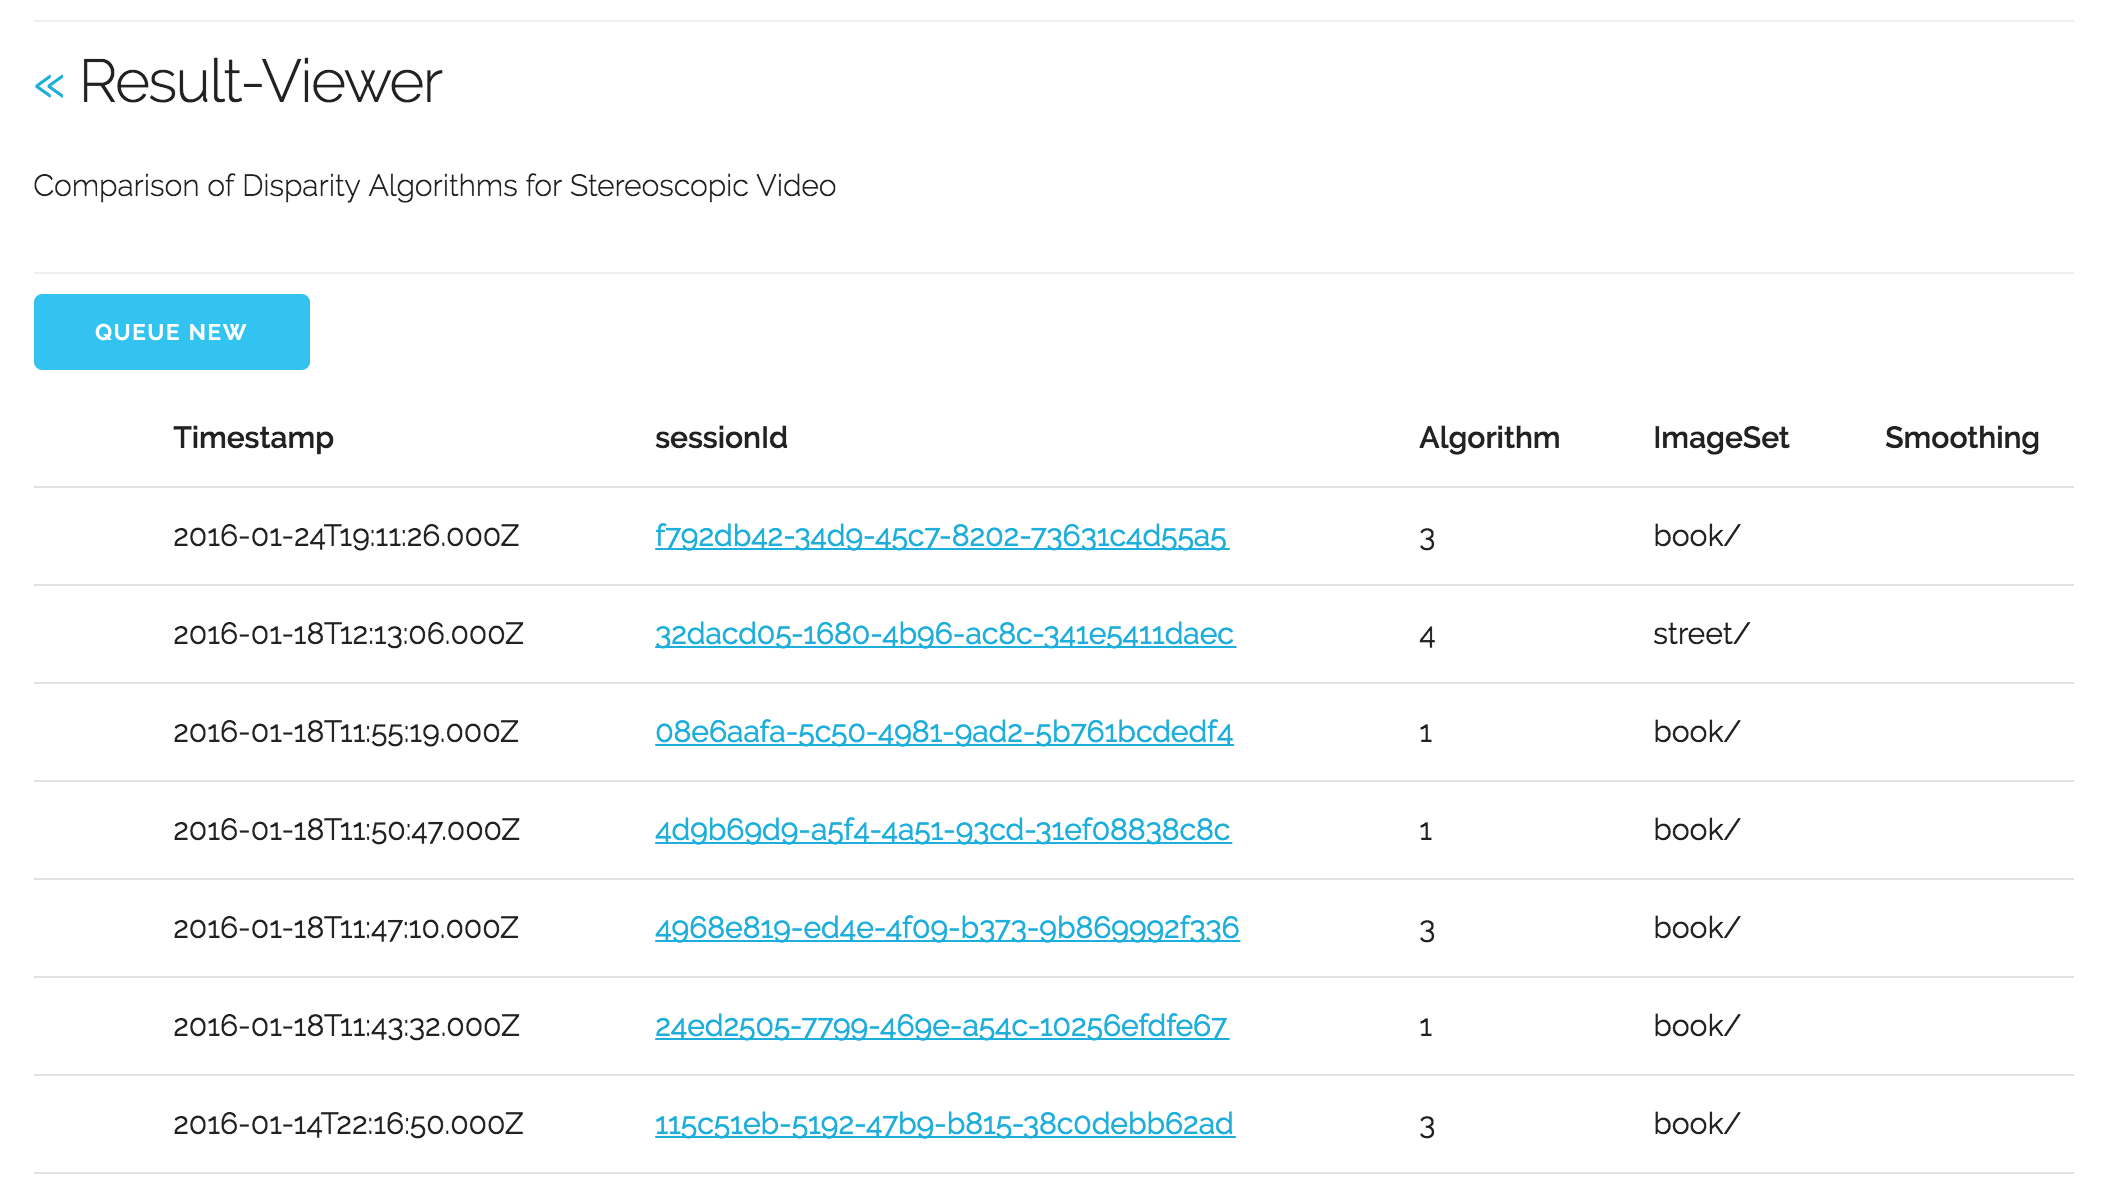
\includegraphics[angle=90,width=0.7\textwidth]{src/images/result-viewer-overview.png}
  \caption{Overview page of web result viewer.}
  \label{fig:web-overview}
\end{figure}

\begin{figure}[p!]
  \centering
  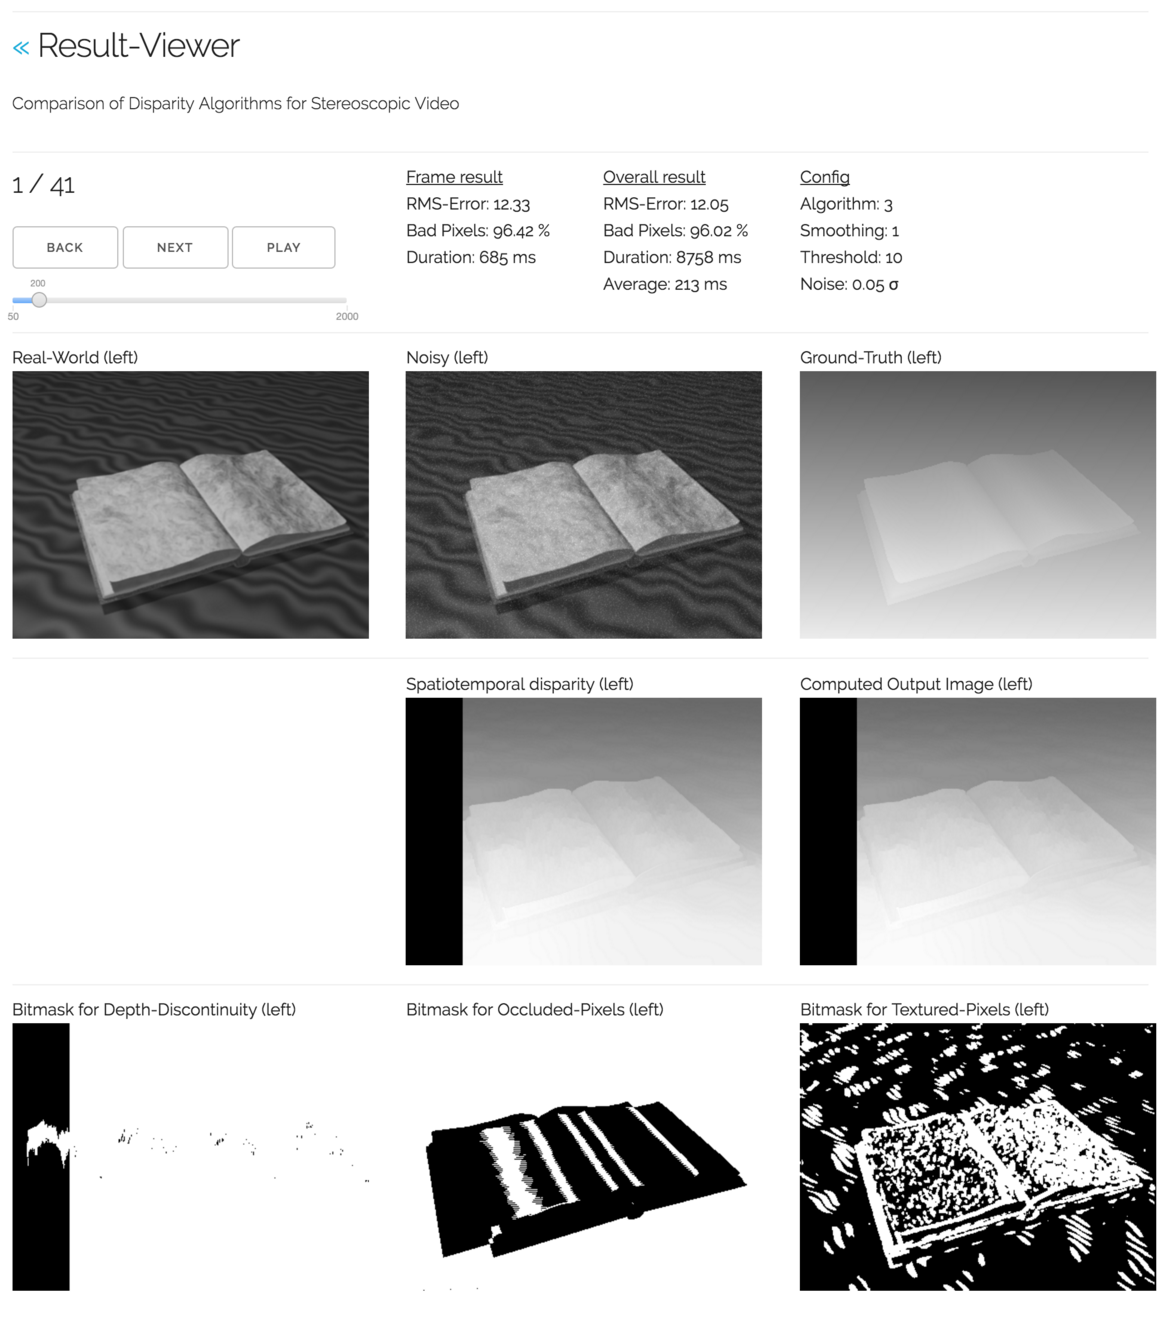
\includegraphics[angle=90,width=1.0\textwidth]{src/images/result-viewer-detail.png}
  \caption{Detail of one result in the web result viewer.}
  \label{fig:web-detail}
\end{figure}

%todo finish web result viewer section
\begin{itemize}
  \item Insert screenshot (one or two from web result viewer)
  \item Describe basic features
  \item Describe what could be done with the evaluation web suite in near future
  \item But for thesis evaluation a csv exporter was used.
\end{itemize}

\section{Discussion}

The following modules were actually implemented:

\begin{itemize}
  \item Reader for the PFM file format.
  \item Python scripts for upcoming evaluation.
  \item Shell scripts for getting the docker containers and thus the work distributed among different instances\footnote{With instances virtual machines from DigitalOcean are meant.}.
  \item Evaluation processor for
\end{itemize}
